\documentclass{beamer}

\usepackage{comment}
\usepackage{color}
\usepackage{listings}
\usepackage{verbatim}
\usepackage{multicol}
\usepackage{booktabs}
\usepackage{textpos}
\usepackage{graphicx}
\usepackage{graphics}
\definecolor{green}{RGB}{0,128,0}

\newcommand\gehcomment[1]{{{\color{orange} #1}}}
\newcommand\add[1]{{{\color{blue} #1}}}
\newcommand\remove[1]{\sout{{\color{red} #1}}}
\newcommand\codecomment[1]{{{\color{green} #1}}}
\newcommand\redcomment[1]{{{\color{red} #1}}}
\newcommand\bluecomment[1]{{{\color{blue} #1}}}
\newcommand\greencomment[1]{{{\color{green} #1}}}
\newcommand\magentacomment[1]{{{\color{magenta} #1}}}

\begin{document}
\title{Multi-Well\ldots}
\author{Michael Nole}
\date{\today}

%\frame{\titlepage}

%-----------------------------------------------------------------------------
\section{Description of Multi-Well Scenario}

\subsection{Multi-Well Conceptual Model}

\frame{\frametitle{Description of Multi-Well Scenario}

The ``Multi-Well Scenario'' simulates an injection well and an extraction well in 3D in \bluecomment{SCO2 MODE}. The injection well alternately injects CO2 and water at a prescribed schedule. The extraction well follows a different schedule. Both wells are prescribed flow rates subject to fracture pressure and minimum pressure limitations.

This demonstration covers the following:

\begin{itemize}
  \small
  \item Set up a 3D model with two fully coupled hydrostatic wells in SCO2 mode.
  \item Run the simulation.
  \item Visualize results in Paraview.
\end{itemize}
}

%-----------------------------------------------------------------------------
\section{Description of Input Deck}

%-----------------------------------------------------------------------------
\subsection{DESCRIPTION}

\begin{frame}[fragile,allowframebreaks]\frametitle{DESCRIPTION}

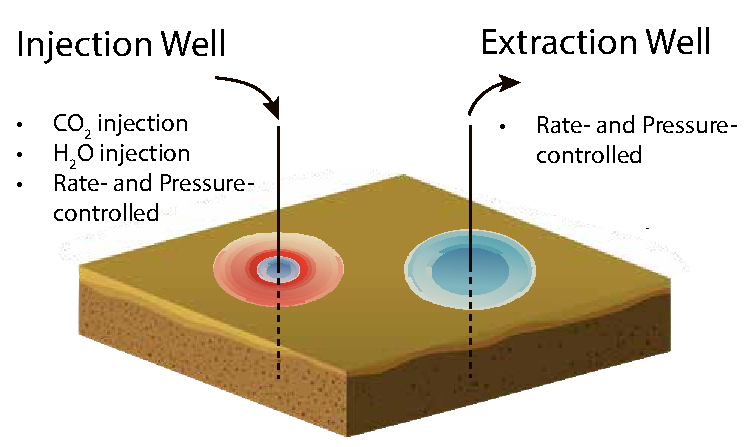
\includegraphics[height=3in]{multi-well-fig.pdf}

\newpage
\begin{itemize}
  \item 1. Initialize to hydrostatic conditions. Optional: turn on \bluecomment{ISOTHERMAL\_GRADIENT}
  \item 2. Injection schedule: 0.5 MMT/yr CO2 for 3 years, 0.1 MMT/yr H2O for 7 years.
  \item 3. Fracture pressure threshold: 15 MPa
  \item 4. Extraction schedule: At 1 year, extract at 0.1 MMT/yr for 19 years.
  \item 5. Minimum pressure threshold: 2 MPa
\end{itemize}

\end{frame}

%-----------------------------------------------------------------------------
\subsection{SIMULATION\_MULTI-WELL}

\begin{frame}[fragile,allowframebreaks]\frametitle{SIMULATION: Multi-Well}
\begin{semiverbatim}
SIMULATION
  SIMULATION_TYPE SUBSURFACE
  PROCESS_MODELS
    SUBSURFACE_FLOW flow
      MODE SCO2
      OPTIONS
        NO_STATE_TRANSITION_OUTPUT
        \bluecomment{#ISOTHERMAL_GRADIENT}
      /
    /
\newpage
    WELL_MODEL well
      OPTIONS
        FLOW_COUPLING FULLY_IMPLICIT
        TYPE HYDROSTATIC
      END
    END
  /

END

SUBSURFACE
...

\end{semiverbatim}

\end{frame}

%-----------------------------------------------------------------------------
\subsection{NUMERICAL METHODS}
\begin{frame}[fragile]\frametitle{NUMERICAL METHODS}
\begin{semiverbatim}
NUMERICAL_METHODS flow

  NEWTON_SOLVER
    USE_INFINITY_NORM_CONVERGENCE
    NUMERICAL_JACOBIAN
    MINIMUM_NEWTON_ITERATIONS 2
    CONVERGE_ON_WELL_RESIDUAL
  END

  TIMESTEPPER FLOW
    TIMESTEP_MAXIMUM_GROWTH_FACTOR 1.25
  END

END

\end{semiverbatim}
\end{frame}

%-----------------------------------------------------------------------------
\subsection{WELL MODEL}
\begin{frame}[fragile,allowframebreaks]\frametitle{WELL MODEL}
\begin{semiverbatim}
WELLBORE_MODEL injector
  PRINT_WELL_FILE
  WELL_GRID
    WELL_TRAJECTORY
      SURFACE_ORIGIN 775.d0 775.d0 2.d2
      SEGMENT_LIST FILE injector_well-segments.dat
      \bluecomment{#SEGMENT_DXYZ CASED 0.d0 0.d0 -100.d0}
      \bluecomment{#SEGMENT_DXYZ UNCASED 0.d0 0.d0 -80.d0}
    /
  /

\newpage
  WELL
    DIAMETER 0.3d0
    FRICTION_COEFFICIENT 1.d0
    WELL_INDEX_MODEL PEACEMAN_3D
    SKIN_FACTOR 0.d0
  /

  FRACTURE_PRESSURE 1.5d7

  USE_WELL_COUPLER

END
\newpage
WELLBORE_MODEL producer
  PRINT_WELL_FILE
  WELL_GRID
    WELL_TRAJECTORY
      SURFACE_ORIGIN 1225.d0 1225.d0 2.d2
      SEGMENT_LIST FILE producer_well-segments.dat
      \bluecomment{#SEGMENT_DXYZ CASED 0.d0 0.d0 -100.d0}
      \bluecomment{#SEGMENT_DXYZ UNCASED 0.d0 0.d0 -80.d0}
    /
  /
\newpage
  WELL
    DIAMETER 0.3d0
    FRICTION_COEFFICIENT 1.d0
    WELL_INDEX_MODEL PEACEMAN_3D
    SKIN_FACTOR 0.d0
  /

  MINIMUM_PRESSURE 2.d6

  USE_WELL_COUPLER

END
\newpage
WELL_MODEL_OUTPUT
  WELL_LIQ_PRESSURE
  WELL_GAS_PRESSURE
  WELL_LIQ_Q
  WELL_GAS_Q
/

\end{semiverbatim}
\end{frame}
%-----------------------------------------------------------------------------
\subsection{GRID}
\begin{frame}[fragile,containsverbatim]\frametitle{GRID}

\begin{itemize}
  \item Cartesian grid, converted to an unstructured implicit mesh.
\end{itemize}

\begin{semiverbatim}
GRID
 #40(50m) x 40(50m) x 20(10m)   
  TYPE UNSTRUCTURED  mesh.ugi
END
\end{semiverbatim}

\end{frame}
%-----------------------------------------------------------------------------
\subsection{FLUID\_PROPERTIES}
\begin{frame}[fragile,containsverbatim,allowframebreaks]\frametitle{Fluid Properties}

\begin{itemize}
  \item Define properties of water and gas
  \begin{itemize}
    \item Diffusion coefficients
    \item Equations of state
  \end{itemize}
\end{itemize}

\begin{semiverbatim}
FLUID_PROPERTY
  PHASE LIQUID
  DIFFUSION_COEFFICIENT 2.d-9
END

FLUID_PROPERTY
  PHASE GAS
  DIFFUSION_COEFFICIENT 2.d-5
END

\newpage

EOS WATER
  DENSITY IF97
  ENTHALPY IF97
  STEAM_DENSITY IF97
  STEAM_ENTHALPY IF97
  SATURATION_PRESSURE IF97
END

EOS GAS
  CO2_DATABASE ../../../../../database/co2_sw.dat
  HENRYS_CONSTANT DEFAULT
END

\end{semiverbatim}

\end{frame}
%-----------------------------------------------------------------------------
\subsection{MATERIAL\_PROPERTY}

\begin{frame}[fragile,containsverbatim,allowframebreaks]\frametitle{MATERIAL\_PROPERTY}

\begin{semiverbatim}
MATERIAL_PROPERTY caprock
  ID 1
  CHARACTERISTIC_CURVES reservoir
  POROSITY 0.1
  TORTUOSITY 1.d0
  ROCK_DENSITY 2650.d0
  THERMAL_CONDUCTIVITY_DRY 2.d0
  THERMAL_CONDUCTIVITY_WET 2.18d0
  HEAT_CAPACITY 1000 J/kg-C
\newpage
  PERMEABILITY
    PERM_X 1.0e-18
    PERM_Y 1.0e-18
    PERM_Z 1.0e-19
  /
  SOIL_COMPRESSIBILITY_FUNCTION LINEAR
  POROSITY_COMPRESSIBILITY 1.0e-10
  SOIL_REFERENCE_PRESSURE 5.d6
END 
\newpage
MATERIAL_PROPERTY reservoir
  ID 2
  CHARACTERISTIC_CURVES reservoir
  POROSITY 0.1
  TORTUOSITY 1.d0
  ROCK_DENSITY 2650.d0
  THERMAL_CONDUCTIVITY_DRY 2.d0
  THERMAL_CONDUCTIVITY_WET 2.18d0
  HEAT_CAPACITY 1000 J/kg-C
\newpage
  PERMEABILITY
    PERM_X 1.0e-14
    PERM_Y 1.0e-14
    PERM_Z 1.0e-15
  /
  SOIL_COMPRESSIBILITY_FUNCTION LINEAR
  POROSITY_COMPRESSIBILITY 1.0e-10
  SOIL_REFERENCE_PRESSURE 5.d6
END
\end{semiverbatim}

\end{frame}

%-----------------------------------------------------------------------------
\subsection{CHARACTERISTIC\_CURVES}

\begin{frame}[fragile,containsverbatim, allowframebreaks]\frametitle{CHARACTERISTIC\_CURVES}
\begin{semiverbatim}
CHARACTERISTIC_CURVES reservoir
  SATURATION_FUNCTION BROOKS_COREY
    UNSATURATED_EXTENSION
    ALPHA 1.d-3
    LAMBDA 2
    LIQUID_RESIDUAL_SATURATION 0.1
    MAX_CAPILLARY_PRESSURE 1.d9
  /
\newpage
  PERMEABILITY_FUNCTION BURDINE_BC_LIQ
    PHASE LIQUID
    LAMBDA 2
    LIQUID_RESIDUAL_SATURATION 0.1
  /
  PERMEABILITY_FUNCTION MODIFIED_COREY_GAS
    PHASE GAS
    LIQUID_RESIDUAL_SATURATION 0.1
    GAS_RESIDUAL_SATURATION 0.2
  /
END
\end{semiverbatim}

\end{frame}

%-----------------------------------------------------------------------------
\subsection{OUTPUT}

\begin{frame}[fragile,allowframebreaks]\frametitle{OUTPUT}

\begin{semiverbatim}

OUTPUT
  SNAPSHOT_FILE
    TIMES d 14.d0
    TIMES y 1.d-2 1.d-1 1.d0
    PERIODIC TIME 1.d0 y
    FORMAT HDF5
  /
  UNFILTER_NON_STATE_VARIABLES
\newpage
   VARIABLES
   TEMPERATURE
   LIQUID_PRESSURE
   GAS_PRESSURE
   LIQUID_SATURATION
   GAS_SATURATION
   PRECIPITATE_SATURATION
   LIQUID_MASS_FRACTIONS
   GAS_MASS_FRACTIONS
   LIQUID_DENSITY
   GAS_DENSITY
   PERMEABILITY
   LIQUID_RELATIVE_PERMEABILITY
   GAS_RELATIVE_PERMEABILITY
  /
END
\end{semiverbatim}

\end{frame}

%-----------------------------------------------------------------------------
\subsection{TIME}

\begin{frame}[fragile]\frametitle{TIME}

\begin{itemize}
\item Run simulation to 10 y
\end{itemize}

\begin{semiverbatim}

TIME
  FINAL_TIME 3.d1 y
  INITIAL_TIMESTEP_SIZE 1.d0 s
  MAXIMUM_TIMESTEP_SIZE 1.d0 y
  MAXIMUM_TIMESTEP_SIZE 9.d-5 y at 1.d0 y
  MAXIMUM_TIMESTEP_SIZE 1.d0 y at 1.0001d0 y
  MAXIMUM_TIMESTEP_SIZE 1.d-2 y at 3.d0 y
  MAXIMUM_TIMESTEP_SIZE 1.d0 y at 3.01d0 y
END

\end{semiverbatim}

\end{frame}

%-----------------------------------------------------------------------------
\subsection{REGION}

\begin{frame}[fragile,containsverbatim,allowframebreaks]\frametitle{REGION}

\begin{itemize}
  \item Delineate regions in the 2D domain for:
  \begin{itemize}
    \item caprock
    \item north, south, east, west boundaries
    \item entire domain
  \end{itemize}
\end{itemize}

\begin{semiverbatim}
REGION all
  COORDINATES
    0.d0    0.d0    0.d0
    1.d20   1.d20   1.d20
  /
END
\newpage

REGION caprock
  COORDINATES
    0.d0 0.d0 1.8d2
    1.d20 1.d20 2.d2
  /
END

\newpage

REGION north
  FACE NORTH
  FILE mesh_ugi_north.ss
END

REGION south
  FACE SOUTH
  FILE mesh_ugi_south.ss
END

\newpage
REGION east
  FACE EAST
  FILE mesh_ugi_east.ss
END

REGION west
  FACE WEST
  FILE mesh_ugi_west.ss
END

\end{semiverbatim}

\end{frame}

%-----------------------------------------------------------------------------
\subsection{FLOW\_CONDITION}

\begin{frame}[fragile,allowframebreaks]\frametitle{FLOW\_CONDITION}

\begin{itemize}
\item Initialize with hydrostatic pressure, geothermal gradient, constant salinity.
\item Specify injection and production schedules.
\end{itemize}

\newpage
\begin{semiverbatim}
FLOW_CONDITION initial
  TYPE
    LIQUID_PRESSURE HYDROSTATIC
    CO2_MASS_FRACTION DIRICHLET
    SALT_MASS_FRACTION DIRICHLET
    TEMPERATURE DIRICHLET
  /
  DATUM 0.d0 0.d0 1.d2
  GRADIENT
    TEMPERATURE 0.d0 0.d0 -2.d-2
  /
  LIQUID_PRESSURE 5.0d6
  CO2_MASS_FRACTION 1.d-4
  SALT_MASS_FRACTION 1.d-2
  TEMPERATURE 45.d0
END 
\newpage FLOW_CONDITION injection
  SYNC_TIMESTEP_WITH_UPDATE
  TYPE
    RATE MASS_RATE
    TEMPERATURE DIRICHLET
  /
  TEMPERATURE 30.d0
  # 0.5 MMT/yr CO2 for 3 yr
  # 0.1 MMT/yr H2O for 7 yr
  RATE LIST
    TIME_UNITS y
    DATA_UNITS kg/y kg/y kg/y MW
    0.d0  0.d0 5.d8 0.d0 0.d0
    3.d0 1.d8 0.d0 0.d0 0.d0
    10.d0 0.d0 0.d0 0.d0 0.d0
  /
END 
\newpage
FLOW_CONDITION production
  SYNC_TIMESTEP_WITH_UPDATE
  TYPE
    RATE MASS_RATE
  /
  # 0.1 MMT/yr total mass (CO2 + H2O) produced for 19 yr
  RATE LIST
    TIME_UNITS y
    DATA_UNITS kg/y kg/y kg/y MW
    0.d0   0.d0 0.d0 0.d0 0.d0
    1.d0  -1.d8 0.d0 0.d0 0.d0
    20.d0  0.d0 0.d0 0.d0 0.d0
  /
END
\end{semiverbatim}

\end{frame}

%-----------------------------------------------------------------------------
\subsection{INITIAL\_CONDITION}

\begin{frame}[fragile]\frametitle{INITIAL\_CONDITION}

\begin{semiverbatim}
INITIAL_CONDITION all
  FLOW_CONDITION initial
  REGION all
END

\end{semiverbatim}

\end{frame}

%-----------------------------------------------------------------------------
\subsection{BOUNDARY\_CONDITION}

\begin{frame}[fragile,allowframebreaks]\frametitle{BOUNDARY\_CONDITION}

\begin{itemize}
\item Couple the \greencomment{injection} flow condition with well model \greencomment{injector}, \greencomment{production} flow condition with well model \greencomment{producer}, and all boundary conditions with their corresponding faces.
\end{itemize}

\begin{semiverbatim}
WELL_COUPLER injection
  FLOW_CONDITION injection
  WELL injector
END

WELL_COUPLER producer
  FLOW_CONDITION production
  WELL producer
END
\newpage
BOUNDARY_CONDITION north
  FLOW_CONDITION initial
  REGION north
END

BOUNDARY_CONDITION south
  FLOW_CONDITION initial
  REGION south
END
\newpage
BOUNDARY_CONDITION west
  FLOW_CONDITION initial
  REGION west
END

BOUNDARY_CONDITION east
  FLOW_CONDITION initial
  REGION east
END
\end{semiverbatim}

\end{frame}

%-----------------------------------------------------------------------------

\subsection{STRATA}

\begin{frame}[fragile]\frametitle{STRATA}

\begin{semiverbatim}

STRATA
  REGION all
  MATERIAL reservoir
END

STRATA
  REGION caprock
  MATERIAL caprock
END

END_SUBSURFACE
\end{semiverbatim}

\end{frame}

%-----------------------------------------------------------------------------
\subsection{buoyant-flow.in}

\begin{frame}[fragile]\frametitle{Running PFLOTRAN}

\begin{semiverbatim}

> cd \$PFLOTRAN_DIR
> cd shortcourse/exercises/co2/sco2/multi-well
> ./build_grid.sh
> mpirun -n 4 pflotran -input_prefix multi-well
> python plot_wells.py
> paraview \&

\end{semiverbatim}

\end{frame}
\end{document}
